\section{Pipeline}
In this section we elaborate on the full algorithmic pipeline in respect to the sections as described in the previous sections. By combining isometric compression, association vectors, machine learning, phase space projections, and filters we are able to accomplish a novel approach toward data analysis which allows for two important properties: Classification and identification of stable shapes in phase space and a smooth transition between topological and graph structures. This section will demonstrate the component flow in specificsand the full pipeline. Some of the specific techniques used such as clustering, cuts, entropy measures, etc will be proposed in the following sections, however the best implementation of each pipeline component needs to be tested rigorsly and often may be application based.

See Figure 10.2 for the pipeline. 

\begin{figure*}
  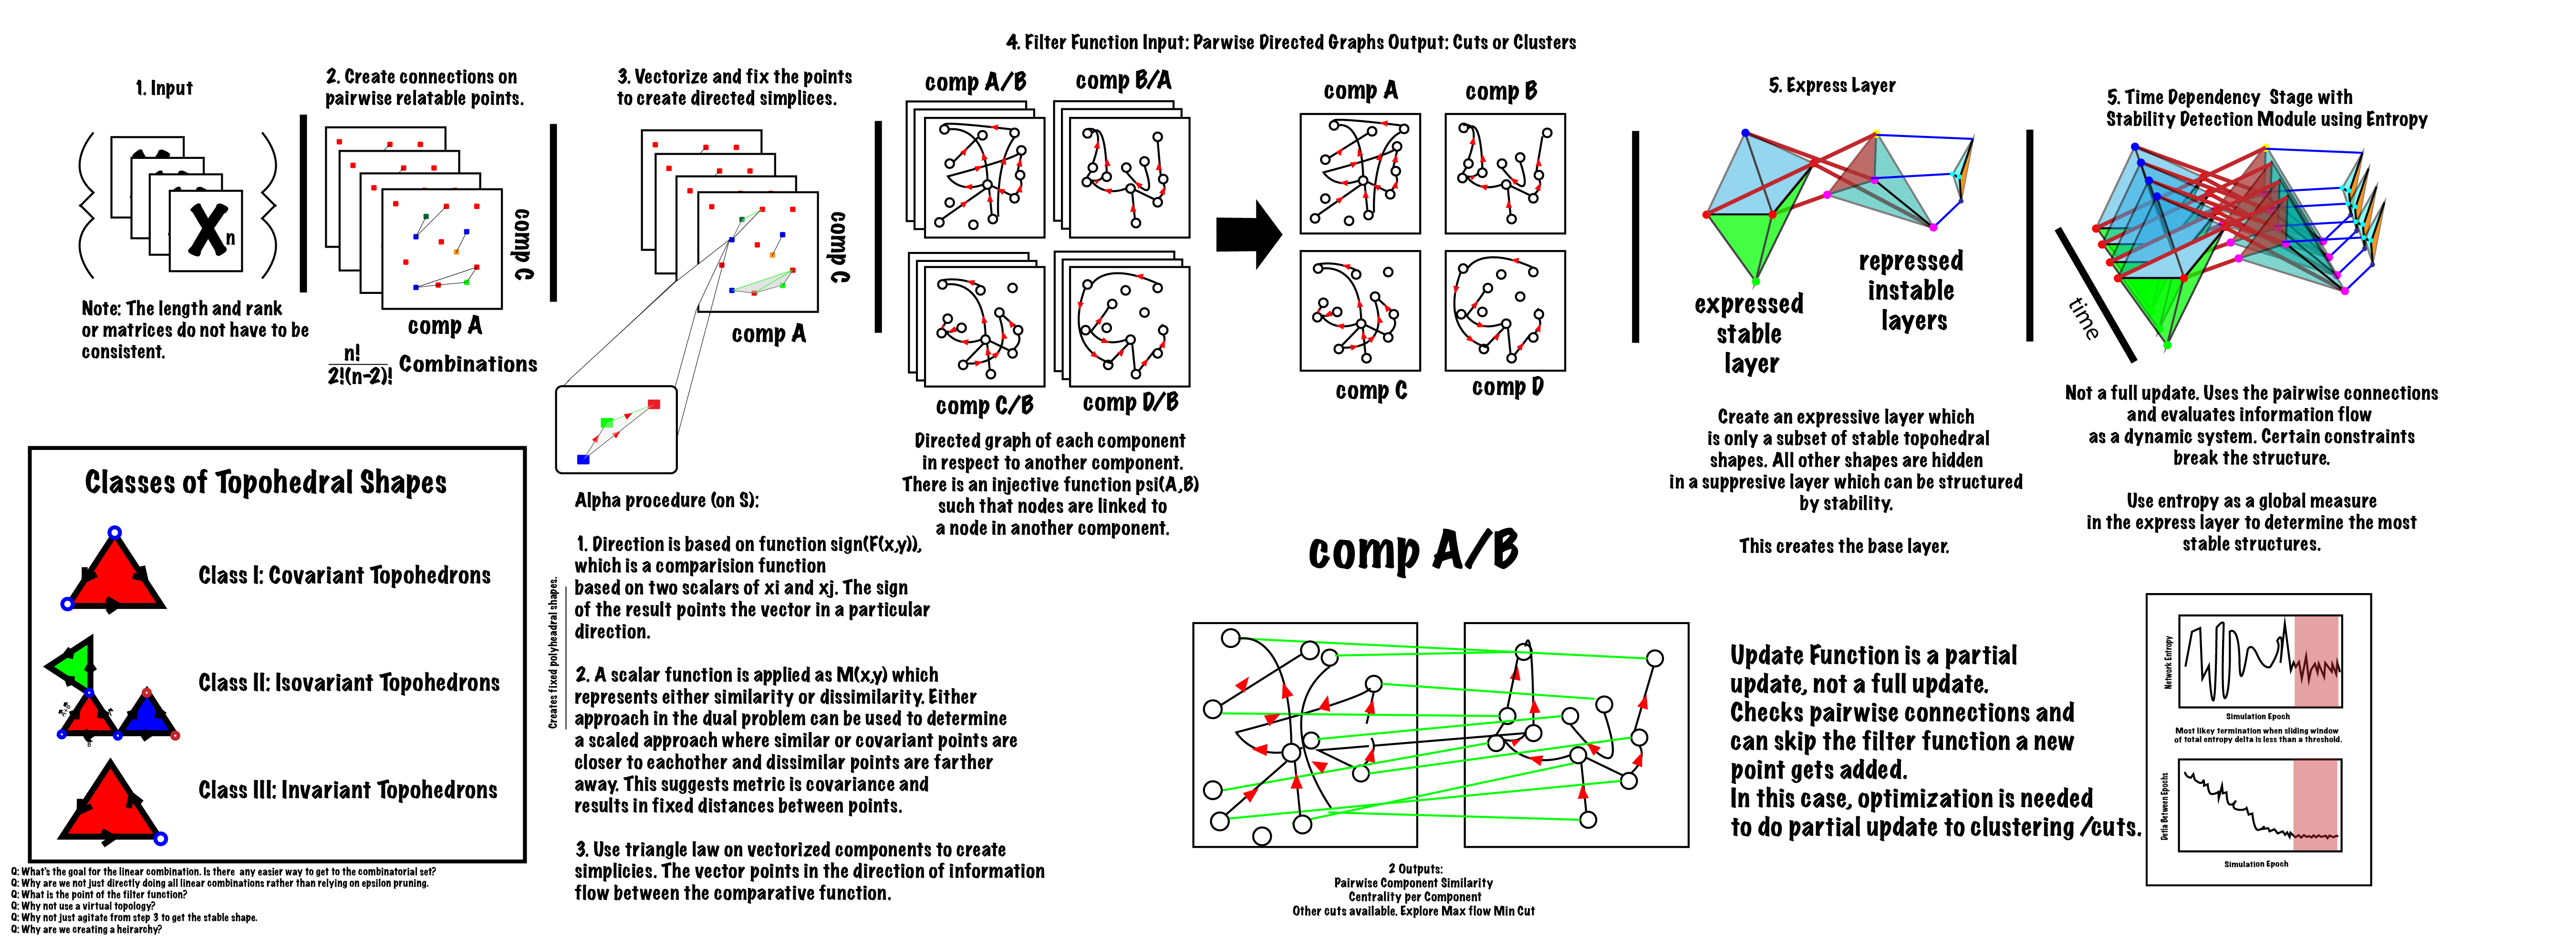
\includegraphics[width=\textwidth]{images/pipeline3}
  \caption{Pipeline}
\end{figure*}
\subsection{Step 0: Input Space}

Let $\mathbb{X}$ or the \textit{Input Space} be superset that consists of a set of $n \times m$ input matrices $X$ where $X_i = [0,N] \subseteq \mathbb{R}^d$ whose union into $\mathbb{X}$ form the toplogical set . The set of $X$ form a topological set $\tau$, due to the following properties:

\begin{itemize}
\item $X \in \tau, \emptyset \in \tau$
\item $\{O_i\}_{i \in I} \subseteq \tau \Rightarrow \bigcup_{i \in I}O_i \in \tau$ (the union of $\tau$ is in $\tau$)
\item $\{O_i\}_{i \in I}^n \subseteq \tau \Rightarrow \bigcap_{i \in I}O_{i=1}^n \in \tau$ (intersections in $\tau$ are in $\tau$)
\end{itemize}

The topological space forms a generalization of the metric space and so any metric space as an input would be sufficient to continue the problem. Due to some of our later constructions in the pipeline it is necessary that there is a bijective mapping $\psi$ for each component within $\tau$ such that $\forall \psi: x \in X \rightarrow y \in X_{y \neq x}$. Moreover, $\forall \cup_{i=0}^n x \in X$ it is one-to-one and forms $X$.   

\subsection{Step 1: Association Vectors}

From point $p \in X$ and set $S \subseteq X$ we denote the minimum distance $\epsilon$ and $\delta(p,S)$ to be the minimum distance function from $p \rightarrow S$. Similar to Vietoris–Rips complex, we evaluate all points within $\delta(p,S) \leq \epsilon$, by drawing them as connected components.

Computationally, creating the connected components is the quadratic of the points in each layer however \footcite{Piegl} there has been a variety of work done to make Vietoris–Rips approximations more computationally tractable such as Donald Sheely who achieves simplicial complexity of $O(n \log n)$ time, however we will leave future papers to discuss optimization strategies necessary for fast computation as this will require modification of traditional Vietoris–Rips constructions. 

Let us call the set connected chain $C$ whose properties include:
\begin{itemize}
\item $C \in X$ and $C \leq X$
\item $\mathbb{C} = \bigcup_{i \in I} C$ such that the union of all connected chains are the set of all connected components.
\item $\| \vec{c} \|$ denotes the length of the connected component, which is the number of edges.
\item $\| \vec{c} \| = n - 1$ where n is the connected vertices.
\item $\|\cap C_{i \in I} / \mathbb{C} \| \geq 0$ such that the intersection of all connectd chains is greater than or equal to 0. 
\item Each component in $C$ can be represented by their pairwise components such that $C_{i,j}$ represent the connection between $C_{i,j}$
\item Order invariant such that $C_{j,k} = C_{k,j}$ 
\item $\mathbb{C} = \{C_{j,k} \rightarrow C_{k,i} \rightarrow C_{i,l} \rightarrow ...\}$ such that $\mathbb{C}$ represents a connected chain which contains no disjoint components. In other words, one could trace the chain without ever having to lift his/her pencil.
\end{itemize}

To encode direction and magnitude into our pairwise connected components, we define the \textbf{Alpha Function} as stated below. 

\begin{definition} [Alpha function]
\end{definition}

Let the $\alpha$ function be an encoding function on a connected set $C$ such that $\forall(c \in C)$, there is a direction and magnitudal component such that $\forall C, (m,d \in c)$. We call each $c$ an association vector which after encoding is denoted as $\vec{c}$. Let the set $\vec{A}$ be bijective and $\vec{A} = C$ however let $C$ be a more generalized form. We call the encoding function $\alpha$, such that $\alpha(C)$ provides the necessary encodings for each vector. There are a number of consequences with this encoding, such as the fact that $\|\vec{c}\|$ is fixed and contingent to the $\alpha$ function.

In dynamic systems, these values change as the data underneath changes, thereby these values are only snapshot invariant. With perterbation to the data and time our underlying encoding undergoes state changes. As will be clear later, this is important to consider because we will use techniques to determine stable structures under pertebation and time.

\textbf{$\alpha_M$: Magnitude Function of Alpha}

Let the magnitude function be consistent with the definition of a distance function, who's length is inversely porportional to the distance encoding. Such is that larger distances are localized with further seperation and closer distances are more proximal with eachother. Let further formulization be described as below:

\begin{enumerate}
  \item $D(A_{a,b}, B_{c,d}) > 0$
  \item $D(A_{a,b}, B_{c,d})$ is finite.
  \item $D(A_{a,b}, B_{c,d})$ is ordinal with higher similarity being inversely porportional to the value.
  \item The relative encodings are scale invariant.  
\end{enumerate}  

\textbf{$\alpha_D$: Directional Function of Alpha}

Let the directional function be a singleton choice in the set $B = \{Source,Target,\emptyset\}$ where the directional component represents flow of information between source and target. For the encoding, we declare a comparitive interface $\alpha_{D}(source,target)$ which chooses an element in B which provides the directional component of the association vector. To measure information flow, we will typically use the function:  $sign(f(source,target))$ where f is a comparative function that measures information flow between the source and the target. 

  \begin{figure}[H]
  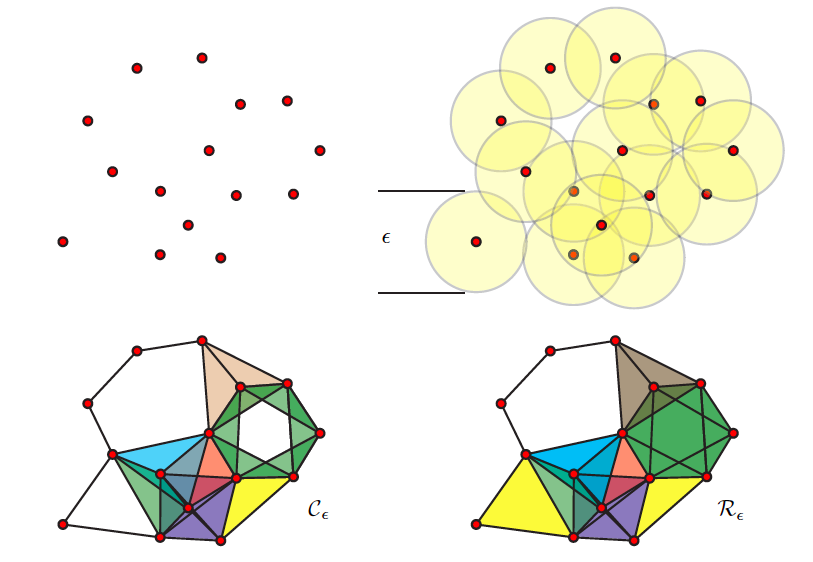
\includegraphics[width=\linewidth]{images/vrcomplex}
  \caption{A fixed set of points. Top right: Closed balls of radius $\epsilon/2$ centered at the points. Bottom left: Cech complex has the homotopy type of the $\epsilon/2$ cover. $(S^1\vee S^1\vee S^1)$ Bottom right: Vietoris-Rips complex has a different homotopy type $(S^1\vee S^2)$. Image from R. }
  \label{vrcomplex} 
\end{figure}

\subsection{Step 2: Directed Simplicial Complex}

\par Using the concept of collinearity, we can create a constrainted and directed simplex by use of the triangle law. We will term each 2-simplex as a "Roy Simplex" and the directed simplicial complex that will eventually be formed after the pipeline is finished as a "Roy Topoheadron". 

\begin{definition}[Roy Simplex]
  Let a roy simplex be a directed simplicial complex where one side is directed vector made from the collinear combination of the two other vectors that compose the 2-simplex.
\end{definition}
  Let a triangle be completable if it can be represented by a linear combination between two vectors in vectorspace. As a basis for this completion, we will use the simple vector triangle law to create collinear connected components. We represent this by equation 10 below. Using another comparative function, we look at the information flow between collinear points to provide a direction for the connecting vector. We will call this this collinear association vector, and this vector is critical for later on in the pipeline for creating stable structures.

\begin{figure}[H]
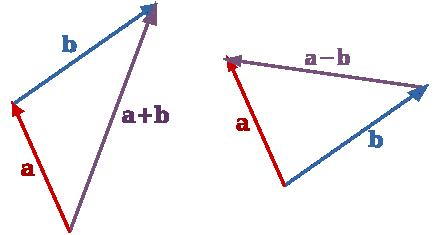
\includegraphics[width=\linewidth]{images/vectoraddition}
\caption{Vector Addition. The left is tail-head oriented vectors. To the right is coinitial vectors}
\label{vectoraddition} 
\end{figure}

\textbf{Triangle of Vector Law Addition}
\newline
If CoInitial Vectors:
\begin{equation}
      \vec{c} = \vec{a} - \vec{b} 
\end{equation}\newline
If Tail-Tail Vectors:
\begin{equation}
      \vec{c} = \vec{a} + \vec{b} 
\end{equation}
where:\\
$\vec{c}$ is the connecting vector between vectors a and b, originating at a singleton if it is coinitial.
If the vectors are tail-head oriented then $\vec{c}$ originiate from different points. 
\par We term the \textit{Dominating Vector} to be larger magnitude of two vectors |A| and |B|. To find the dominate vector is very simple. The formulate $sign(\|\vec{a}\| - \|\vec{b}\|)$ gives the dominate vector with respect to the first component. When providing direction to our generated vector, we point the vector towards the dominate vector. This is intended to mimic the flow of information from one point to another.

The generated vector we term as the \textbf{dependent vector}.

\subsubsection{Roy Simplex Classifications}

Let us denote the information state of the network as $W$ and the velocity of the information toward the beginning and end of each timestep as $W_i$ and $W_f$ respectively. Let us denote $\Delta(W)$ as the total change of information in the network through over timestep $h$ and $\partial(W)$ to be related to the component differentials of $W$.

The formation of Roy Simplicial Complexes and ostensibly Roy Polyhedrons have geometric implications that will be described below. We classify the roy simplex into three different classifications based upon the intrinsic nature of the simplex.

\textbf{[Class I] - Invariant Topohedrons:} are topohedrons that perserve symmetry under all cases. They are formed as a colinear combination of two vectors and are stable structures in the topohedron. As the flow of information changes between the dependent vector, the structure is stable and the toplogy does not change.   

\textbf{[Class II] - Covariant Topohedrons:} are topohedrons that perserve symettry however are linked simplicials on a single vertex. 

\textbf{[Class III] - Isovariant Topohedrons:} are formed by cycles in information flow and thus have no dominate vector. There are few properties unique to an isovariant topohedron. 


\begin{figure}[H]
  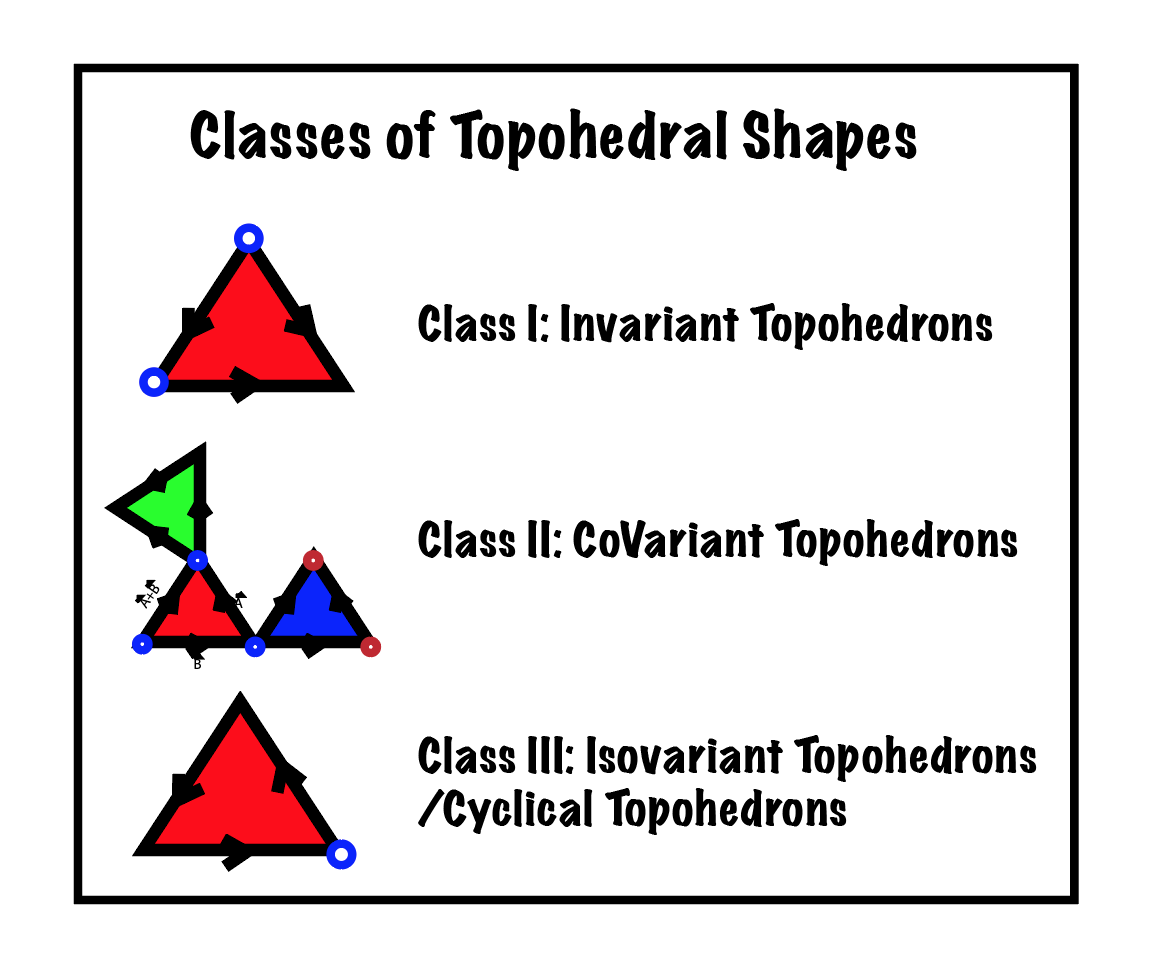
\includegraphics[width=\linewidth]{images/classes}
  \caption{Classes Explained} % Figure caption
  \label{classes} 
\end{figure}

\subsection{Express Steps}
\begin{definition}[Component Map]
  Let $\psi: A \rightarrow B$ be the component map from component A to component B which is an injective map between pairwise components. 
\end{definition}
Let us call the express step in the pipeline a lossy compression step where we isometrically compress the simplicial simplices formed in Step 3 into multi-level classifications. To do this, we employ partial clustering on filter mechanisms such as centrality and pairwise simlarity to form cardinality on the set. We use the highest rank of cardniality to form the set we call the \textit{Express Layer} and follow the expressed layer by disjoint sets called \textit{Repressed Layers}.

After filtration, three componential "Roy Simplexes" and connected to form a "Roy Topoheadron". The Roy Topoheadron has a number of special properties.

\subsection{Entropy Measurements and Stability Detection}
As a dynamic system, we can produce these "Roy Topoheadrons" over time, which allow us to monitor the development of the topology through phase space. We define the phase space of a roy topoheadron to be the shadow projection of the topological shape over time. By using a measurement of network entropy. 

Gibbs Entropy
\begin{equation}
\sigma = 1/N log \digamma
\end{equation}

where: $\digamma$ denotes the cardinality of the ensemble. Other measurements include metrics such as:\\
\newline

\begin{center}
  \textbf{Shannon Entropy}: $S = (\mathcal{L}) = - \sum_{i<j} \sum_{\alpha} \pi_{ij}(\alpha)log\pi_{ij}(\alpha) $
\end{center}
There is more work to be done to find the best entropy measurements for a dynamic system of directed topological objects and graphs. \footcite{Bianconi2009}

\subsection{Updating Topology}
Our update function does not need to recompute all steps from scratch. There are a variety of opimization steps that can be employed to increase the efficieny of update function. After the first run, we can optimize so each step updates minimalistic. The optimizations will be discussed in a seperate paper. 
